%!TEX root=../mythesis.tex
% Chapter 1

\chapter{Introduction} % Main chapter title
\chaptermark{Introduction}
\label{ch:introduction} % For referencing the chapter elsewhere, use \ref{Chapter1} 

%----------------------------------------------------------------------------------------
%	SECTION 1
%----------------------------------------------------------------------------------------

%\section{Some useful hints}
%
%My figure citation: \fref{fig:demo1}. (command: fref)
%
%My section citation: \sref{sec:contribution}. (command: sref)
%
%My Chaptere citation: \cref{ch:introduction}. (command: cref)
%
%My Paper citation: \cite{bauschke2011convex}. (notice back reference to page from bibliograph)
%
%My equation citation: \eqref{eq:equ2}. (command: eqref), or cite equation by tag: \eqref{eq:equ1}.
%
%\begin{equation}\label{eq:equ1}
%F(\theta)=\sum_{i=1}^mf_i(\theta) \tag{DOP}
%\end{equation}
%
%\begin{equation}\label{eq:equ2}
%F(\theta)=\sum_{i=1}^mf_i(\theta)
%\end{equation}
%
%\begin{figure}[htbp]
%  \centering
%    
\includegraphics[width=0.85\textwidth]{Chapter1/demo1}
%  \caption{An illustration.}
%  \label{fig:demo1}
%\end{figure}

%
Deep learning, a sub-field of machine learning capable of learning higher-dimension feature representations via neural networks and gradient descent, has attracted remarkable attention from researchers over the last few decades.
%
Landmark works in deep learning, for example, the first attempt of using GPUs in training neural networks~\cite{krizhevsky2012imagenet}, the introduction of the self-supervised training technique capable of mapping words to representation space~\cite{mikolov2013efficient}, or the introduction of the Transformer architecture~\cite{vaswani2017attention}, have actively and significantly driven the deep learning research community forward. 
%
On the one hand, the ability to recognize patterns presented in and extract information from a large amount of data, without relying on handcrafting rules and heuristics, has made deep learning methods incredibly powerful and attractive.
%
On the other hand, countless applications of deep learning have been developed in many aspects of our lives, from vision tasks such as facial recognition~\cite{masi2018deep}, image restoration~\cite{gao2017demand}, natural language tasks such as machine translation~\cite{stahlberg2020neural}, speech recognition~\cite{kumar2019comprehensive}, to more complex decision-making tasks such as autonomous driving~\cite{kiran2021deep} or healthcare treatment administration~\cite{yu2021reinforcement}.

\section{Question Answering}
\label{sec:qa}

\begin{figure}[!htbp]
	\centering
	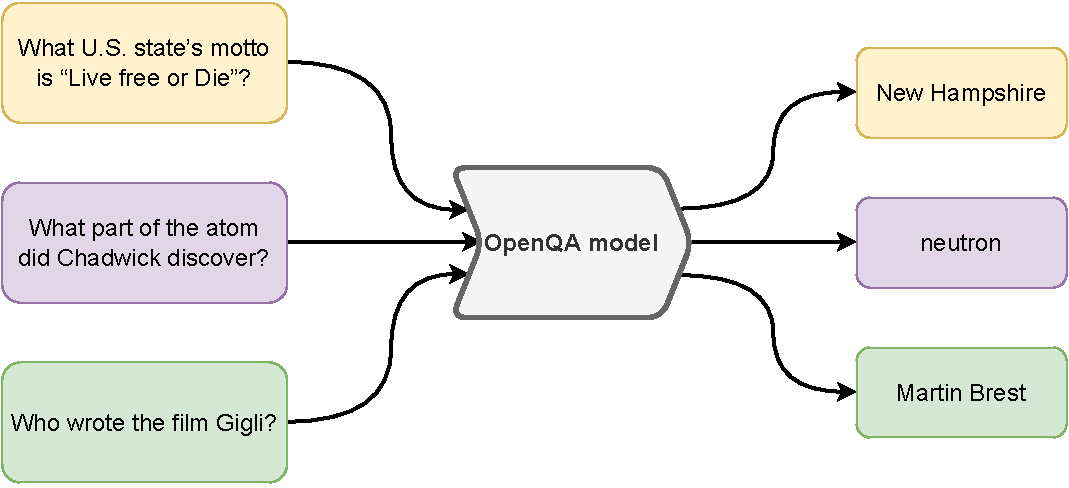
\includegraphics[width=0.7\linewidth]{introduction/openqa.pdf}
	\caption[Examples of input-output pairs in open-domain question answering.]{
		%
		Examples of input-output pairs in open-domain question answering (OpenQA).
		%
		The goal of OpenQA is to answer any factoid question about nearly anything. Adapted from~\cite{chen2020open}.
	}
	\label{fig:openqa}
\end{figure}


%
Question answering (QA), a naturally arisen task that aims at answering questions posed by humans, has generally received great attention thanks to the wide range of real-world applications that it offers.
%
However, most of the previous works on QA have mainly placed their focus on closed-domain question answering and machine reading comprehension (MRC).
%
While closed-domain QA limits the questions being asked to a specific domain knowledge (e.g., medicine), or to a specific type of questions (e.g., \emph{when}), MRC systems are allowed to read and comprehend relevant context passages in order to answer the questions.
%
In contrast, the long-standing problem of open-domain question answering~\cite{voorhees1999trec} (OpenQA) has observed significantly less progress, potentially due to its complex and large-scale nature.
%
Open-domain question answering is a much more challenging task than closed-domain QA or MRC as it requires cutting-edge techniques from both natural language processing (NLP) and information retrieval (IR).
%
In OpenQA, the model must answer any factoid questions, possibly about anything, without being provided relevant contexts containing the answer.
%
\fref{fig:openqa} illustrates several examples of input-output pairs in OpenQA.
%
Notably, OpenQA can be utilized in a wide range of applications, ranging from online customer service systems, chatbots (e.g., Siri) to search engines (e.g., Google), where user inputs are usually information-seeking questions.
%
With OpenQA, we aim at developing intelligent systems that automatically retrieve and extract relevant information of a given question, and subsequently suggest a detailed answer.

\section{Closed-book and Open-book Open-domain Question Answering}
\label{sec:close_and_open_book}

%
OpenQA can be further classified into two categories, namely closed-book OpenQA and open-book OpenQA.

\subsection{Closed-book Open-domain Question Answering}
\label{sec:close_book}
%
In closed-book OpenQA, the system is not given access to any textual documents when answering the questions, and thus is expected to memorize factual knowledge ahead of time stored implicitly in its parameters (\emph{parametric memory}).
%
At test time, the system is expected to provide answers to questions that it has already encountered during training by
retrieving from its memory, or to infer answers to unseen questions using general ontologies and common
knowledge.
%
This is analogous to a student memorizing possible question-answer pairs from a set of past year papers before coming to a closed-book final examination.

%
Despite its simplicity and straightforward formulation, there exists a number of inherent weaknesses in closed-book OpenQA systems.
%
First, closed-book OpenQA models, which are generative models by design, have been long known to suffer from \emph{factual hallucination}~\cite{ji2022survey}.
%
Factual hallucination is a common phenomenon in text generation in which the models fail to precisely retrieve factual information from their parametric memory, and thus unintendedly attempt to fabricate it.
%
Such unfaithful behaviors should obviously be avoided in question answering where precise fact is of utmost importance.
%
Second, closed-book OpenQA systems generally require a huge number of parameters to accommodate their parametric memory, which often far exceeds the amount of storage used to store factual knowledge in plain text.
%
For example, a state-of-the-art closed-book OpenQA system~\cite{roberts2020much} is only able to match the performance of a recent open-book OpenQA system~\cite{karpukhin2020dense} while requiring 11 times as many parameters.
%
Third, it is not trivial to update closed-book OpenQA models with new information (for example recent events), as it would require re-training the models.
%
This in turn gives rise to the \emph{catastrophic forgetting} problem~\cite{kemker2018measuring}, another common issue in deep learning in which the model loses its generalizability and catastrophically forgets existing knowledge after being trained on new data.

\subsection{Open-book Open-domain Question Answering}
\label{sec:open_book}
%
Open-book OpenQA has been proposed to tackle the aforementioned issues that closed-book OpenQA suffers from. 
%
At inference time, an open-book OpenQA system is provided access to a large knowledge base, for example Wikipedia articles, from which it can search for supporting passages to the given question.
%
This formulation allows the system to retrieve precise factual knowledge from the non-parametric memory of passages, effectively overcoming the factual hallucination and catastrophic forgetting problems.
%
At the same time, the number of parameters can be significantly reduced given that the models no longer have to memorize information by storing it in the parameters.
%
Finally, such non-parametric knowledge source as Wikipedia is human interpretable and can be easily updated.
%
Given these advantages, in this work, we mainly tackle the problem of open-book OpenQA and simply refer to it as~\emph{OpenQA}  for brevity.


\begin{figure}[!htbp]
	\centering
	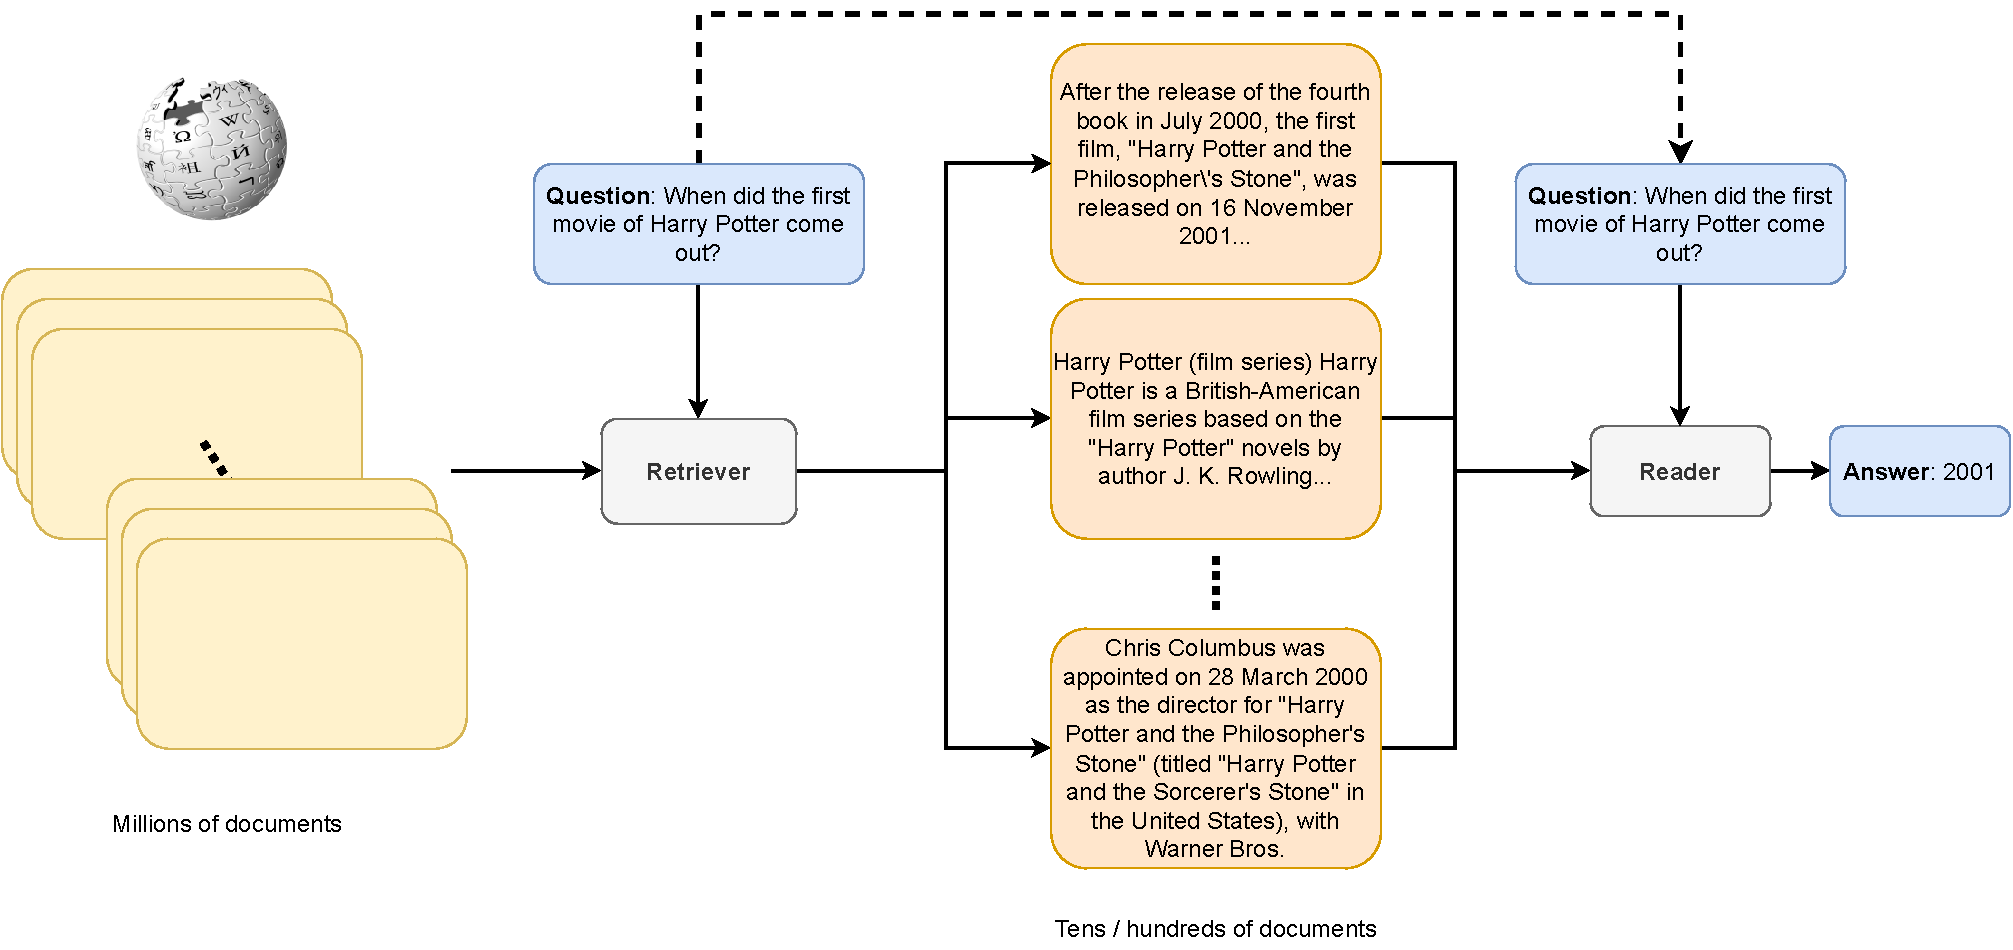
\includegraphics[width=0.95\linewidth]{introduction/open_book_openqa.pdf}
	\caption[An overview of the two-stage retriever-reader model.]{
		%
		An overview of the two-stage retriever-reader model.
		%
		The retriever first performs a highly efficient search algorithm to retrieve top-$k$ most relevant passages from a large collection of documents (e.g., Wikipedia).
		%
		The reader then reads this subset of documents to infer the answer to the given question.
	}
	\label{fig:open_book_openqa}
\end{figure}


%
It is important to highlight that we are processing millions of documents in open-book OpenQA given a single input query.
%
Thus, it would be computationally infeasible to naively apply machine reading comprehension to every passage in the corpus and return the most probable answer.
%
To overcome this challenge,~\citet{chen2017reading} proposed a two-stage~\emph{retriever-reader} paradigm that has gained popularity recently due to its effectiveness and efficiency.
%
\fref{fig:open_book_openqa} presents an overview of this approach.
%
In the first stage of this framework, a small number of relevant passages is retrieved by a \emph{retriever} model using a highly efficient search algorithm.
%
A~\emph{reader} model is then used to perform reading comprehension on this subset of passages to obtain the final answer.
%
Analogously, in an open-book exam, the students should first identify relevant sections in the
textbooks before actually delving into the details to find answers to a given question, instead
of reading every paragraph one by one looking for the solutions.

%
In~\citet{chen2017reading}, a simple TF-IDF~\cite{jones1972statistical} weighted bag-of-words method is used as the retrieval method while an LSTM-based~\cite{hochreiter1997long} model is employed as the MRC method.
%
The retrieval method, which belongs to a family of non-trainable~\emph{sparse retrieval} approaches, performs a simple and efficient word matching step to find relevant passages.
%
On the other hand, the reader model has a limited capability of understanding long sequences, be it the forgetfulness in RNN-based models or quadratic time complexity in Transformer-based models~\cite{devlin2019bert}.
%
Since the introduction of the two-stage paradigm, many advances in Natural Language Processing (NLP) have been proposed to push the boundary of OpenQA systems further, especially the retriever model.
%
\citet{lee2019latent} and~\citet{guu2020realm} adopted trainable~\emph{dense retrieval} models, which are first pre-trained in an unsupervised manner before being fine-tuned on the downstream OpenQA data.
%
\citet{seo2019real} combined the complementary advantages of sparse retrieval and dense retrieval in a unified framework.
%
\citet{khattab2020colbert} aimed to address a key challenge in dense retrieval, namely the \emph{decomposability gap} which we will introduce shortly, with vector decomposition and late interaction to mimic the self-attention~\cite{vaswani2017attention} mechanism.
%
Dense Passage Retrieval (DPR)~\cite{karpukhin2020dense} later showed that pre-training is not needed for dense retrieval as the retriever model directly trained on OpenQA data with in-batch negatives and the negative log-likelihood (NLL) objective function significantly outperformed all other approaches.

%
In all of the previous algorithms, the query and passage texts will first be compressed into some vectorized form in order to enable a highly efficient search algorithm on the retriever side.
%
For sparse retrieval, the documents are encoded with weighted word frequency, for which severe information loss will incur such as the loss of sequential information and semantic meaning of the texts.
%
On the other hand, for dense retrieval, information compression is done by mapping each sequence of words to its high-dimensional vector representation.
%
Not only does this approach benefit from the advantages of representation learning from supervised data, but it also enables the use of the well-studied, highly efficient Maximum Inner Product Search (MIPS)~\cite{johnson2019billion} algorithm.
%
Notably, regardless of the retrieval type, the computational cost of extracting information from the knowledge base can be further amortized by pre-computing and pre-indexing it into a MIPS index.
%
As a result, at test time, we only need to compress the input question (e.g., by feeding it through the dense retriever model to obtain its vector representation) before sending it to the MIPS index for efficient retrieval of relevant passages.
%
This procedure effectively reduces the number of passages for the reader model from millions of documents to 50-100 documents in real-time.
%
However, it also inevitably limits the ability of the model to capture mutual information between the passages and the input questions (so-called the \emph{decomposability gap}).
%
As discussed above, this is to some extent caused by the loss of information during the data compression step, even for dense retrievers.
%
Moreover, it is important to note that the evidence documents and the input query are encoded independently of each other.
%
Thus, the task of the retrievers is to find the best passage matches to a given question when both the passages and the question have already been encoded, without being allowed to comprehend the original texts.
%
In other words, decomposability gap happens when the computationally expensive reading comprehension task is decomposed into two smaller and efficient tasks of feature representation and maximum inner product search.
%
As a consequence, this performance trade-off significantly negatively affects the relevance of passages retrieved in the first stage, which in turn is detrimental to the reader performance, thus the overall OpenQA performance.

%
Decomposability gap is regarded as the most challenging yet attractive problem in OpenQA.
%
Previous work on mitigating this challenge can be classified into several main directions.
%
To explicitly tackle the decomposability gap, \citet{khattab2020colbert} aimed at mimicking the self-attention mechanism between the passage and the input query via late vector interaction, while~\citet{das2018multi} allowed communication between the retriever and reader to iteratively fine-tune the retrieval results.
%
Another research direction is query expansion, whereby the input query is first augmented with relevant keywords before compression, effectively pushing the representation of this query closer towards that of the gold passages in the feature representation space~\cite{mao2021generation, qi2019answering}.
%
Notably, a large body of works focused on improving the retriever performance with novel pre-training paradigms~\cite{lee2019latent, guu2020realm, lewis2020retrieval, chang2020pre, lewis2020pre, xiong2021progressively}.
%
Lastly,~\citet{seo2019real},~\citet{lee2020contextualized} and~\citet{luan2021sparse} combined the complementary strengths of sparse and dense retrieval to improve the overall retrieval performance.
%
In this final year project, we extend upon the outstanding work Dense Passage Retrieval~\cite{karpukhin2020dense}.
%
We explore the first three aforementioned directions as well as other directions and further propose multiple novel approaches with the main goal of improving the overall OpenQA performance, as well as with a particular focus on the decomposability gap of retrieval.



%%
%\citet{clark2018simple} as well as~\citet{wang2019multi} proposed several techniques to comprehend multiple passages simultaneously, thereby improving the reading comprehension performance while being more efficient.
%%
%Similarly,~\citet{wang2018evidence} proposed various methods to aggregate answers obtained from reading different passages, for example by their weighted frequency.
%%
%\citet{lee2019latent} pre-trained the retriever with Inverse Cloze Task and then jointly fine-tuned the retriever and the reader on OpenQA data.
%%
%\citet{guu2020realm} extended this direction by proposing a better pre-training paradigm called Salient Span Masking and a better joint training approach.
%%
%Dense Passage Retrieval (DPR) showed that 
%%
%\citet{lewis2020retrieval} combined both the pre-training and joint training paradigms 


%%
%This algorithm, which will be described later in more detail in~\FAKEREF{NEED REFERENCE!!}, is orders of magnitude faster than the naive approach, therefore enabling a real-time OpenQA performance.
%%
%However, this architectural design comes with an inherent trade-off, namely decomposability gap, which negatively affects the relevance in the returned documents.


%----------------------------------------------------------------------------------------
\section{Major Contributions}\label{sec:contribution}
Our main contributions can be stated as follows:
\begin{itemize}
\item
%
We propose several simple yet under-explored multi-task learning approaches for OpenQA that yield sizeable performance improvements while reducing the memory footprint of the retriever, which is critical for real-time OpenQA systems.

\item
%
We explore a simple method aimed at capturing the mutual information between the question query and documents during retrieval.
%
This method explicitly considers the decomposability gap and can be seen an alternative to the late interaction mechanism proposed in~\citet{khattab2020colbert}.

\item
%
We propose a simple data augmentation method to diversify the retrieval training data, thereby improving the previous state-of-the-art DPR retriever by a large margin.

\item
%
We investigate the effect of the objective function (so-called loss function) on retrieval training, from which we propose new objective functions for representation learning that achieve marginal gains over the baseline model.

\item
%
Finally, we propose a novel data synthesis - semi-supervised pre-training - query expansion paradigm with the goal of comprehensively improving both the retriever and reader, for which we achieve considerable performance improvements across several benchmarking datasets.


\end{itemize}


%\section{Outline of the Thesis}
%
%\FAKEREF{Work In Progress}

%\cref{ch:introduction} introduces ...
%
%\cref{ch:literature_review} reviews ...
%
%
%
%More chapters ....
%
%
%....

